\section{Backend}
%TODO: @Joshua

\subsection{Aufbau}

Der Aufbau der Serverapplikation lehnt sich am Konzept der Onion-Architecture an.
In Onion Architecture wird die Applikation in Layer aufgeteilt.

\begin{figure}[h]
    \centering
    \begin{minipage}[b]{0.4\textwidth}
        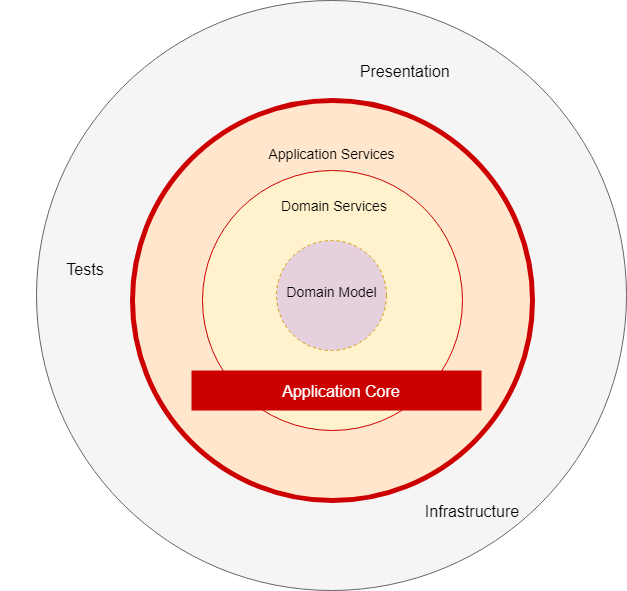
\includegraphics[width=\textwidth]{graphics/thinktocode-onion}
        \caption{Onion Architecture}
    \end{minipage}
\end{figure}

Um zu garantieren, dass keine ungewollten Abhängigkeiten zwischen Layern bestehen, können die Layer in eigene Module verpackt und Abhängigkeiten über Interfaces abstrahiert werden.
Dies erhöht jedoch die interne Komplexität der Applikation.
Die Umsetzung wird aufgrund der geringen Projektgrösse deshalb nicht in unabhängigen Modulen realisiert, sondern über die Package Struktur gelöst.
Angesichts dieser Entscheidung wird weiter darauf verzichtet, Abhängigkeiten zwischen Modulen über Interfaces zu abstrahieren.
Da es nie mehrere Implementationen einer Componente geben wird, bringt der Einsatz von Interfaces keinen grossen Mehrwert.
Bei der Implementation wird dabei konsequent darauf geachtet, die einzelnen Layer so zu halten das diese als eigenständige Module extrahiert werden können.
Für die Verwaltung der Komponenten der Serverapplikation wird folgende Packagestruktur definiert:

\begin{figure}[h]
    \centering
    \begin{minipage}[b]{0.9\textwidth}
        \dirtree{%
            .1 ch.fhnw.woweb.teamdocumentserver.
            .2 config.
            .2 domain.
            .2 persistence.
            .2 service.
            .2 web.
        }
        \caption{Package Struktur Cloud Service}\label{fig:packagescloudservice}
    \end{minipage}
\end{figure}

Der Domain Layer wird durch das Package domain abgebildet.
Dieses beinhaltet die Domänenobjekte und darf keine Abhängigkeiten auf andere Module oder Frameworks beinhalten.
Umgekehrt dürfen alle anderen Layer Abhängigkeiten auf den Domain Layer haben.
Die Fachlogik der Applikation wird im Domain Service Layer implementiert.
Dieser wird durch das Package service abgebildet.
Das Package Service beinhaltet alle Komponenten welche die Domänenobjekte verwalten oder den internen Zustand der Applikation führen.
Der Layer Application Services bildet die Brücke zwischen externer Infrastruktur und Domain Services.
Er ist in den Packages persistence und web beinhaltenagebildet.
Dabei definiert das Package persistence Services welche für Interaktion mit der Datenbank verwendet werden.
Das Package web definiert die HTTP-Endpunkte, welche für die Kommunikation mit dem Frontend des Systems verwendet werden.
Letztlich beinhaltet das Package config die technische Konfiguration der Applikation.

\clearpage

\subsection{API}

Die Backendapplikation bietet eine HTTP-Schnittstelle, welche von Frontendapplikationen verwendet werden kann.
Die Schnittstelle ermöglich es, sich im System anzumelden, Dokumente zu laden und Änderungen an Dokumenten zu laden und speichern.
Um diese Funktionalität zu ermöglichen, bietet die Schnittstelle die drei Bereiche ''Authentication'', ''Document'' und ''Message''.

\subsubsection{API Authentication}

Macht Authentifizierung

\begin{tabbing}
Left \= Middle \= Right \= Right \kill
Endpunkt:  \> \> \> /api/v1/authentication\\
Methode \>  \> \> GET\\
Headers:  \> \>   \> Authentication: Basic \\
Response Code:  \> \>  \> 200, 401 oder 500 \\
Response Body:  \> \>  \> application/json \\
\end{tabbing}

\subsubsection{API Document}

Liefert den Initialen Status und Updates

\begin{tabbing}
    Left \= Middle \= Right \= Right \kill
    Endpunkt:  \> \> \> api/v1/document\\
    Methode \>  \> \> GET\\
    Headers:  \> \>   \> Authentication: Basic\\
    \> \>   \> X-ClientId: text\\
    Response Code:  \> \>  \> 200, 401 oder 500 \\
    Response Body:  \> \>  \> text/event-stream \\
\end{tabbing}


\subsubsection{API Message}

Verarbeitet Updates

\begin{tabbing}
    Left \= Middle \= Right \= Right \kill
    Endpunkt:  \> \> \> /api/v1/message\\
    Methode \>  \> \> POST\\
    Headers:  \> \>   \> Authentication: Basic\\
    \> \>   \> Content-Type: application/json\\
    Body:  \> \>  \> DocumentCommand\\
    Response Code:  \> \>  \> 200, 401 oder 500 \\
\end{tabbing}

Stellt den zuletzt gelöschten Paragraphen wieder her.

\begin{tabbing}
    Left \= Middle \= Right \= Right \kill
    Endpunkt:  \> \> \> /api/v1/message/restore\\
    Methode \>  \> \> POST\\
    Headers:  \> \>   \> Authentication: Basic\\
    Response Code:  \> \>  \> 200, 401 oder 500 \\
\end{tabbing}

\clearpage

\subsection{Komponenten}

\subsubsection{Package Domain}

Im Zentrum der Domäne stehen die beiden Klassen DocumentCommand und Document.

\begin{figure}[h]
    \centering
    \begin{minipage}[b]{0.8\textwidth}
        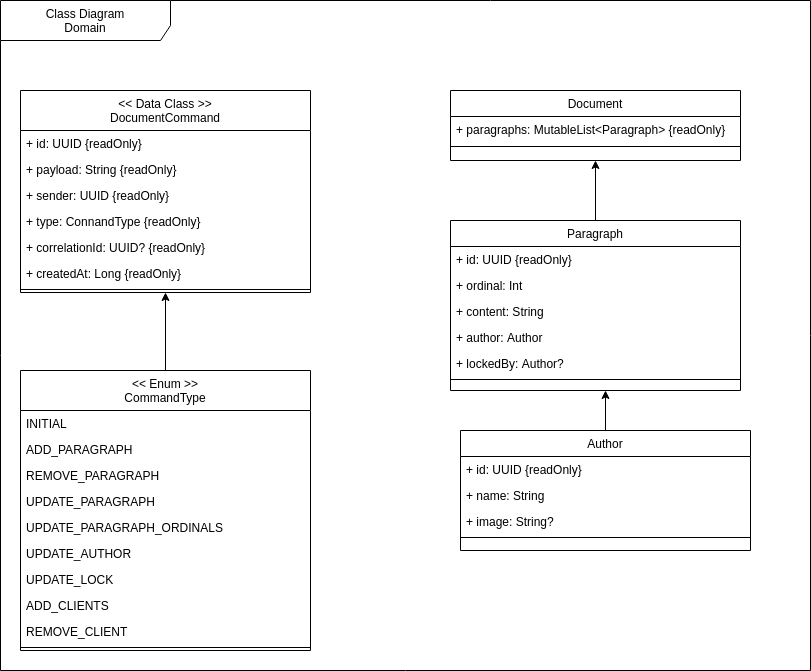
\includegraphics[width=\textwidth]{graphics/class-be-domain.drawio}
        \caption{Klassendiagramm Domain}
    \end{minipage}
\end{figure}

\textbf{Document}

Eine Instanz der Klasse Document repräsentiert den aktuellen Zustand eines Dokuments.
Dieser Zustand wird in der Serverapplikation geführt und verwaltet.
Ein Document besteht im Wesentlichen aus einer Liste von Paragraphs.
Diese Liste kann mutiert, aber nicht ersetzt werden.

\textbf{Paragraph}

Eine Instanz der Klasse Document repräsentiert einen Abschnitt in einem Dokument.
Jeder Paragraph wird durch eine UUID identifiziert.
Ein Paragraph definiert weiter ein Attribut Content welches den Textinhalt des Abschnitts beinhaltet und ein Attribut Ordinal, welches die Position des Abschnitts im Dokument darstellt.
Weiter ist jeder Paragraph einem Author zugewiesen.
Letztlich hat ein Paragraph ein Optionales Attribut lockedBy.
Dieses kann entweder leer (NULL) sein oder einen Author beinhalten.
Dieses Feld kann von Consumern der API verwendet werden um das bearbeiten eines Paragraphen zu erlauben oder verbieten.

\textbf{Author}

Eine Instanz der Klasse Author repräsentiert einen Benutzer, der an einem Dokument mitarbeitet.
Jeder Author wird durch eine UUID identifiziert und muss einen Namen definieren.
Weiter besitzt ein Author ein optionales Attribut image.
Darin kann die URL zu einem benutzerbild abgespeichert werden

\clearpage

\textbf{DocumentCommand}

Eine Instanz der Klasse DocumentCommand stellt eine Änderung am Zustand einer Document-Instanz dar.
DocumentCommands werden als einzige Entität, Persistenzschicht abgelegt werden.
Damit DocumentCommands eindeutig identifiziert werden können, beinhaltet jede Instanz ein Attribut vom Type UUID.
Diese id wird auch als Identifikator in der MongoDB verwendet.

Die Änderungen welche ein DocumentCommand darstellt, werden über die Attribute payload und type definiert.
Die payload hat den Typ String und beinhaltet JSON-Serialisierten des neuen Zustands, er Änderung die vorgenommen werden soll.
Das Feld type beinhaltet einen Wert aus der Enum CommandType.
Dieser Wert kann in den Domänenservices verwendet werden um die Payload korrekt zu Deserialisieren und die nötigen Änderungen am Document vorzunehmen.

Das Optionale Feld correlationId kann entweder NULL oder eine UUID beinhalten.
Eine allfällige UUID zeigt immer auf die Id eines anderen DocumentCommands, welcher mit dem aktuellen Command zusammenhängt.
Dadurch wird es möglich die Identifkation der Payload eines Commands zu verwenden, ohne die Payload jedesmal deserialisieren zu müsen.

\textbf{CommandType}

Bei CommandType handelt es sich um eine Enum.
Diese Enum beinhaltet alle Arten von DocumentCommands, welche im System bekannt sind.
CommandTypes werden als ihr String Wert auf DocumentCommands persistiert.

%INITIAL \\
%ADD\_PARAGRAPH \\
%REMOVE\_PARAGRAPH \\
%UPDATE\_PARAGRAPH \\
%UPDATE\_PARAGRAPH\_ORDINALS \\
%UPDATE\_AUTHOR \\
%UPDATE\_LOCK \\
%ADD\_CLIENTS \\
%REMOVE\_CLIENT \\

\subsubsection{Package Web}

\textbf{AuthenticationController}

Die Klasse AutenticationController implementiert einen RestController.
Dieser stelt einen einzelnen GET Endpunkt zur Verfügung, über welchen sich Benutzer mittels Basic Authentication anmelden können.

\textbf{CommandController}

Die Klasse CommandController implementiert einen RestController.
Dieser Controller bietet zwei POST Endpunkte zur Verfügung.
Über den ersten Endpoint kann eine Liste von DocumentCommands an den Server gesendet werden.
Der Endpunkt übergibt diese Liste von Commands an den DocumentService.
Diese wenden die Änderungen am Zustand des Dokuments an und leiten die Änderungen an andere Teilnehmer weiter.
Über den zweiten Endpunkt kann ein gelöschter Paragraph wiederhergestellt werden.
Die entsprechende Fachlogik wird an den DocumentSerivce delegiert.
%TODO: Generic undo description?

\textbf{DocumentStreamUpdateController}

Die Klasse DocumentStreamUpdateController implementiert einen RestController.
Dieser Controller ermöglicht es, den aktuellen Zustand eines Dokumentes zu laden und Änderungen am Dokument zu abonnieren.
Der Endpunkt, welcher dazu zur Verfügung steht erwartet, dass der Custom Header ''X-ClientId'' gesetht ist.
Dieser muss einen Stringwert beinhalten, welchen den Author der die Daten anfrägt identifiziert.
Das Laden des Dokuments und das Erstellen der Abonnierung wird an den DocumentService delegiert.
Als Rückgabetyp wird ''Flux$<$DocumentCommand$>$ verwendet.
Dadurch ist es möglich den Status des Documents und alle folgenden Änderungen in einem Stream zurückzugeben.

\clearpage

\subsubsection{Package Services}

\begin{figure}[h]
    \centering
    \begin{minipage}[b]{0.8\textwidth}
        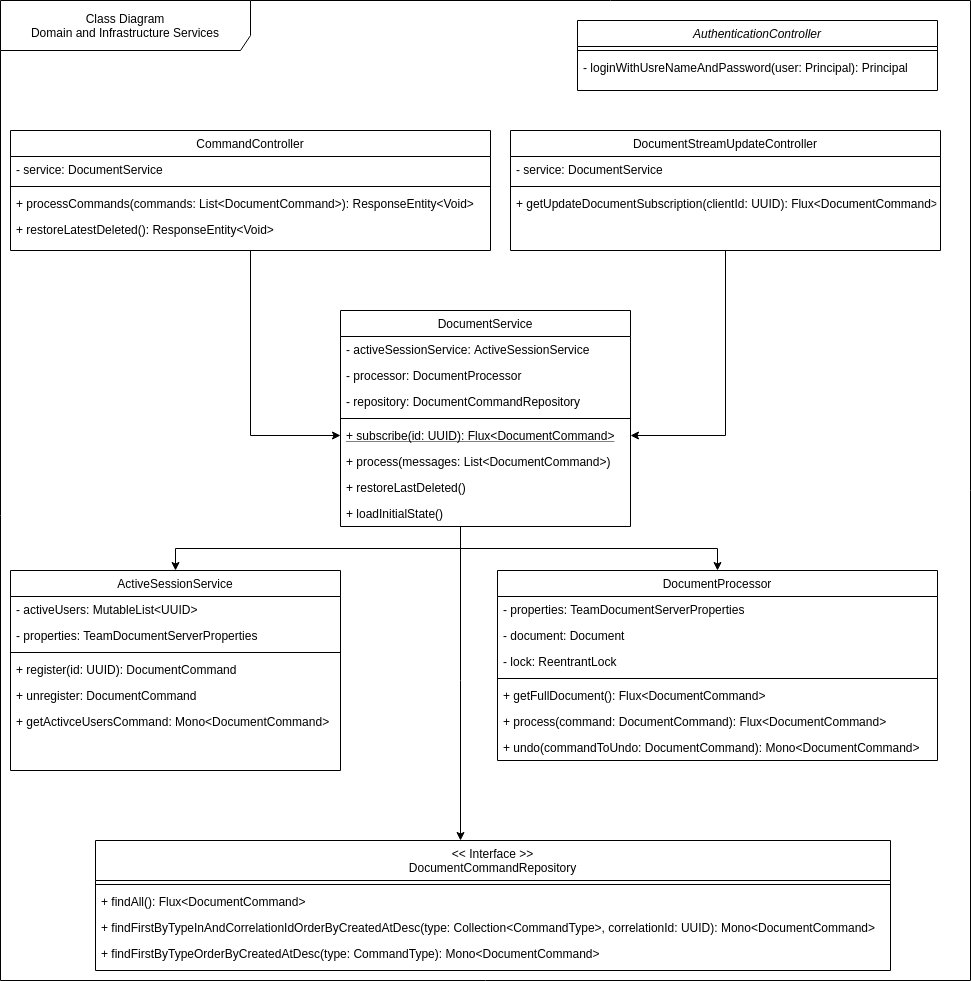
\includegraphics[width=\textwidth]{graphics/class-be.drawio}
        \caption{Klassendiagramm Services}
    \end{minipage}
\end{figure}


\textbf{DocumentService}

Die Klasse DocumentService ist dafür Verantwortlich erhaltene Anfragen für Dokumente und Änderungen an Dokumenten zu verarbeiten.
Sie delegiert die entsprechende Fachlogik Klassen ActiveSessionService, DocumentProcessor und DocumentCommandrepository.

Die Methode process erlaubt es, eine Liste von DocumentCommands zu verarbeiten.
Dabei wird die Verarbeitung an den DocumentProcessor delegiert.
Dieser wendet Änderungen an und löst Konflikte auf.
Die übergebenen Commands und allfällige Commands zur Konfliktlösung werden vom DocumentProcessor zurückgegeben.
Der DocumentService übergibt diese an das DocumentCommandRepository zur persistierung.
Anschliesend werden die Persistierten Commands über den Sink veröffentlicht.

Die Methode subscribe erlaubt es, einen Stream des aktuellen Zustands des Dokuments und aller künftigen Änderungen an einem Dokument anzufragen.
Diese Informationen werden aus drei Quellen zusammengetragen.
Zuerst wird der aktuelle Stand des Dokuments beim DocumentProcessor angefragt.
Anschliessend wird eine Liste aller aktuellen Authoren des Dokuments aus dem ActiveSessionService geladen.
Letztlich wird eine Subscription auf den Sink erstellt.
Diese drei Quellen werden zusammengefasst aus der Methode zurückgegeben.
Um sicherzustellen, dass die Liste der aktiven Nutzer aktuell ist, wird zudem beim Öffnen der Subscription eine Registrierung beim ActiveSessionService durchgeführt.
Diese Registrierung wird beim Schliessen der Subscription wieder entfernt.

\textbf{DocumentProcessor}

Die Klasse DocumentProcessor führt den Zustand des Dokuments, welches mit der Applikation verwaltet wird.
Er ist dafür Verantwortlich, Änderungen an diesem Dokument vorzunehmen.
Dazu besitzt Sie ein Attribut document vom gleichnamigen Typ.
Über die Methode process kann ein einzelner DocumentCommand angewendet werden.
Der Processor verarbeitet denm Command anhand des gesetzten CommandTypes.
Dabei muss er allfällige Konflikte erkennen und auflösen.
Nach der Verarbeitung des Commands werden alle Änderungen und Konfliktlösungen als DocumentCommands zurückgegeben.

\textbf{ActiveSessionService}

Die Klasse ActiveSessionService fürt den Zustand der aktiven Nutzer einer Session.
Dazu führt die Klasse eine Liste der Identifikatoren aller aktiven Nutzer einer Session.
Der Service bietet Methoden um die aktiven Benutzer auszulesen, einen neuen Benutzer zu registrieren und einen Benutzer zu entfernen.

\subsubsection{Package Persistence}

\textbf{DocumentCommandRepository}

Das Interface DocumentCommandrepository erweitert das Interface ReactiveCrudRepository$<$DocumentCommand, UUID$>$ von Spring.
Es kann damit verwendet werden um Create, Read, Update und Delete Optionen für DocumentCommands in der angebundenen MongoDB auszuführen.

\subsubsection{Konfiguration}

\textbf{Spring}

Alle Klassen im Package "Service" sind mit der Spring-Boot-Annotation ''@Service'' versehen.
Sie können damit automatisch von Spring-Boot instanziert werden und stehen Sie in Spring Beans zur Verfügung und können über Constructor-Injection verwendet werden.

Alle Klassen im Package "web" sind mit der Spring-Boot-Annotation ''@RestController'' versehen.
Sie können damit automatisch von Spring-Boot instanziert werden.

\textbf{application.yml}

Die Datei application.yml beinhaltet die konfigurierbaren Werte der Serverapplikation.
Dies beinhaltet die Konfiguration der angebundenen MongoDB, Referenzen zu Umgebungsvariablen mit User Credentials und Logging Konfiguration.

\textbf{TeamDocumentServerProperties}

Die Konfigurationsklasse TeamDocumentServerProperties ist mit der Annotation ''@ConfigurationProperties(prefix = "teamdocument")'' versehen.
Sie kann wo nötig in den Serviceklassen verwendet werden, um auf Werte aus dem application.yaml zuzugreifen.

\textbf{WebConfig}

Die Klasse WebConfig beinhaltet die Konfiguration für SpringSecurity.

\clearpage

\subsection{Sequenz}

\subsubsection{Subscription Öffnen und Schliessen}

\subsubsection{DocumentCommand verarbeiten}

\clearpage

\subsection{State- und Konfliktmanagment}


\clearpage
